\section{九七後的香港政制不是比九七前更民主嗎?}

要評價一個政治體制是否民主,第一要看政府和民意代表是否選舉產生,第二要看選舉的制度和過程是否公開公正。從第一方面看,已不難發現九七後香港的民主有退步;說到第二方面,近年來整個制度的實行更明顯地比九七前不民主。

「九七前的港督由英國委派,九七後的行政長官由選舉產生,首次由香港人擔任」是建制陣營經常起用的說法,以支持他們認為九七後的香港更為民主。這說法的問題是就算當日英國指派一個香港人做總督,不等於英治就不是殖民統治,關鍵在於這個人選是如何產生。事實上,正如很少人會同意北韓的選舉為真正的選舉,所謂的行政長官選舉也不應被視為選舉。由於絕大多數選舉委會員成員都不是由普及的選舉產生,而且和中央政府關係密切,中央政府的支持比香港民意更能決定誰人當選(見問題十八)。林鄭月娥比曾俊華不受歡迎,卻能勝出擔任行政長官,就是實在的證明。再者,九七前被委派的港督尚且會與英國政府持不同意見,今天的行政長官卻只會為站在中央政府的立場向港人說話,以行政長官選舉來說明香港政制變得更為民主,明顯欠缺說服力。

立法機關方面,九七前最後一屆的立法局選舉中,有三十席由功能界別選出,二十席由地區直選選出,另有十席由選舉團產生。九八年特區首屆的立法會的組成表面上一樣,但內容卻大為不同。首先,功能界別的選民基礎大幅收窄,不少組別都由個人票改為團體票,可操控性大幅增加。選舉團方面,一九九五年時由區議員組成,而由於該屆區議會絕大多數議員都是直選產生,可算是一種間接選舉;到了一九九八年時選舉團卻改為由工商界主導的八百人組成,全港大多數選民被一次過排除在選民基礎以外。此外,選舉團議席以全票制而非按得票比例產生,使建制陣營可以囊括所有選舉團議席。這些改變使得首屆立法會的代表性明顯比九七前有所倒退。在傾斜的制度下,建制陣營在選舉中取得優勢,而由於他們往往對政府採合作態度,立法會監察政府的力度也有所降低。由選舉團選出立法會議席的安排,要到了二零零四年的第三屆立法會才完全取消。

提到區議員,區議會在九七後也恢復了委任制。區議會在一九八二年剛成立的時候,民選議員只佔少數,多數為官守和委任議員。到了一九九四年時,官守議席經已取消,政府也放棄行使委任議員的權力。因此除了極少數代表鄉事委員會的當然議員外,其餘所有的區議員都由直選產生。九七後的首屆區議會選舉,特區政府重新恢復委任議員,使區議會的民主成份明顯倒退。區議會委任制要到了二零一六年的區議會選舉中才全面取消。

最後,特區政府於一九九九年解散市政局和區域市政局,嚴重打擊了香港的政制民主。香港原本實行三級議會制,市政局和區域市政局原為中間的一層,處於立法機關和區議會之間。它們負責文娛康樂和環境衛生,例如圖書館管理和街道清潔等功能,擁有自主財政實權及土地使用權。相對於有制度缺陷的立法會和沒有實權的區議會,市政局和區域市政局有更大的空間實踐民主管治。特區政府取消兩局後,原來由民選議員負責的職務改由政府部門(康樂及文化事務署和食物環境衛生署)負責,本身就是一大民主倒退。此外,市政局和區域市政局曾經是民選議員歷練的重要階梯,區議員可以通過競選市政局或區域市政局議員,爭取更多曝光和議政經驗,再晉身立法機關。當市政局和區域市政局被取消後,建制陣營和非建制陣營都因而面對青黃不接的問題。而由於可供競選議席數目的忽然減少,也增加了各黨的內部矛盾,當中以資源明顯較少的非建制陣營更受打擊。

以上僅是從機關、議席數目和選舉制度來衡量九七後的民主倒退,如果從制度配套的宏觀視野出發,則倒退更為明顯。

選舉是民主政治的重要組成部分,但不是有選舉就等如有民主。一場選舉要符合民主原則,應符合數個主要標準:容許不同政見者參選、容許普及而平等的投票權、選舉設置應恆常、秘密和安全,以及提供公平的競爭環境。很可惜,這四方面在九七後都沒有明顯進展,甚至有嚴重倒退。

參選權方面,近年的倒退可謂最為明顯和令人意外的。一直以來,香港的參選權均相當簡單和清晰,只要符合年齡和居留資格,邀交足夠選民聯署和按金即可參選,而且一直都有政見明顯處於社會邊緣的人士成為候選人。不過,自二零一六年立法會換屆選舉開始,即不斷有參選人因政治立場而無法參選,而且審批過程明顯地不公開和不連貫。就在二零一六年立法會換屆選舉,五名參選人各因不同政治立場而被取消資格。其中新界東參選人梁天琦因為選舉主任不相信他「真正改變了他過去主張及支持香港獨立的立場」而被裁定提名無效,儘管他曾以更為明確的立場參與二零一六年初的立法會新界東補選,而當時卻能成功參選為正式候選人。與此同時,政治團體香港眾志在二零一六年換屆選舉時派出羅冠聰參選,獲確認為為正式候選人而且成功當選;但到了二零一八年的立法會港島區補選,同屬香港眾志的周庭卻被取消資格,理由是香港眾志認為香港可通過公投自決是否獨立,儘管這個立場在二零一六年羅冠聰參選時已經存在。

自二零一六年以來多次的取消參選資格事件,在社會中引起廣泛質疑。首先,香港政府自己也承認香港現行法例中並無一項稱為「分裂國家」的特定罪行(《基本法》第一條有規定香港是中國一部分,但《基本法》是憲法性文件,用來規範一般人的行為時要通過本地立法落實;《基本法》第二十三條規定禁止分裂國家應有香港自行立法,而此法至今仍未訂立)。政府以沒有法例規管的言論界線作為剝奪公民政治權利的基礎,對民主制度已是巨大打擊。假如這些參選人本身已因此等罪名被定罪,政府再按既有不容許曾判重刑者參選的制度來否定他們的參選資格,制度上的爭議會少很多。而政府多次禁止過去持相同政見卻成功參選的人士或團體再次參選,也顯示了此做法的不連貫性,同樣有違民主制度講求可以預料的原則。即使政府認為近年香港政治出現新的狀況而要加設限制,也應通過正常的立法途經實施,好讓社會公開辯論是否有此需要,而非由行政部門以鬆緊不明的規則設限。僅是參選權這一項,已可明確得出香港民主倒退的結論。

說到普及而平等的投票權,前文提到的選舉制度問題使大量選民被排除在選舉之外,近年輿論也開始擔心政府會否通過行政安排來限制選民的投票權利。例如政府曾建議縮短投票時間,但由於香港長工時為患,加上低下階層因為工作時間缺乏彈性而未必能在工餘時間前往投票,就並認為會變相剝奪他們的投票權。在二零一六年立法會換屆選舉的投票期間,有個別投票站由於空間不足,選民要排隊數個小時才能投票,最後要等到零晨二時半即原定時間四個小時後才能完成投票,變相排拒時間有限的選民。以類似的方式打壓個別政黨票倉的投票率,在外國有先例可考,輿論也十分關注會否在香港出現。

至於恆常、秘密和安全的選舉,每一方面近年來都受到挑戰。說恆常,過去立法會議員出缺後很快便會安排補選,例如馬力議員於二零零七年八月八日病逝,補選即安排於二零零七年十二月二日舉行,相距四個月;當湯家驊議員於二零一五年十月一日辭職,補選即安排於二零一六年二月二十八日舉行,相距四個月。不過二零一八年三月的補選安排,則被輿論批評為政府固意拖延,甚至有政治考慮。觸發該次補選的議員取消資格案,終極上訴已於二零一七年八月二十五日審結,但補選卻安排於二零一八年三月十一日進行,相距超過六個月。更不幸的,是有建制陣營的代表提議進一步延遲選舉日期,以便他們的成員於北京出席會議,赤裸裸地以黨派利益向選舉程序施壓。

秘密方面,儘管香港法例規定投票保密,亦不可使用通訊或拍攝器材,每次選舉都會傳出有投票人被要求在投票前把已蓋章的選票拍攝下來,以作為投票支持個別候選人的證明。這些傳言固然難以證實,但變相記名投票卻確實在第二屆行政長官選舉和第二屆行政長官繼任選舉中發生。兩次選舉都是由八百人的選舉委員會產生,並規定參選人要取得一百人提名方能成為候選人。結果董建華和曾蔭權分別取得了714人和710人提名,完全排除其他參選人的出線機會下自動當選。當時輿論批評這樣的結果等於把選舉變成記名投票,選委被迫通過提名北京認同的參選人來表示忠誠(見問題十八)。有意見提出要為參選人提交的提名數目設立上限,但政府至今仍未修改相關規定。唯一的修改,是在只有一名候選人的情況之下,仍然要投「支持」和「不支持」,候選人的「支持」票要過半才能當選。

安全方面的倒退,同樣是近年香港政治一個十分意外的發展。所謂安全,是指無論投票、參選或競選活動都可在安全的環境下進行。例如如果通往投票站的路上有軍人、警察或流氓恐嚇選民,就不能稱為民主選舉。香港的情況,集中在候選人和競選活動的安全問題。針對政治人物宣傳品如海報和橫額的破壞,早已司空見慣。在二零一六年的立法會,更接連發生了候選人被恐嚇的事件。新界西候選人周永勤於在競選期間於電視論壇宣布棄選,理由是不想支持他的人「惹上較高層次的麻煩」或付上代價。及後他在記者會中表示在棄選前一天曾到深圳與三名來自北京的人士會面,被警告要立即停止選舉工程,以免其親朋要負上沉重代價。這些人更讀出其親友的詳細個人資料,以施加壓力。同屆另一位候選人朱凱廸,則懷疑因競選期間針對新界土地問題和黑幫的關係,而被黑幫發出死亡恐嚇,警方派出探員全天候保護其家人,並拘捕多名黑幫成員。

\begin{figure}[htbp]
    \centering
    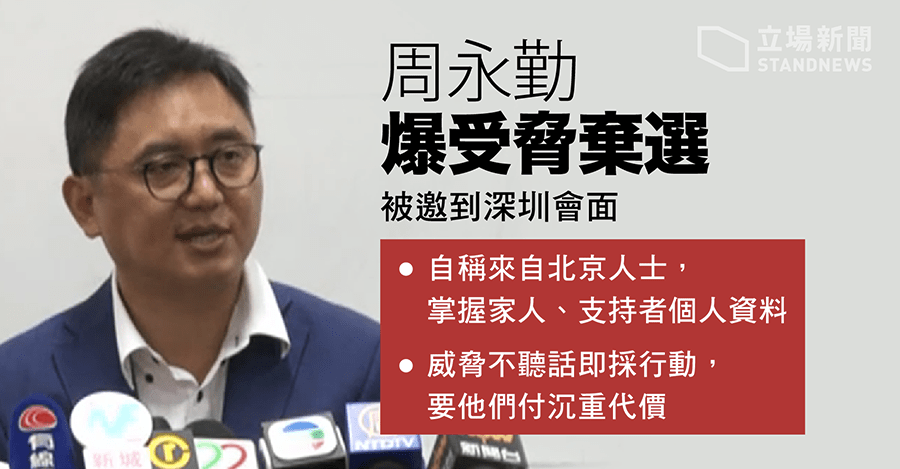
\includegraphics[width=0.7\textwidth]{c33/h-klesson1-054.png}
    \caption{2016年立法會選舉爆出被迫退選事件} 
\end{figure}

至於不公平競爭,則主要體現在政治捐獻之上。傳媒近年多次揭發中聯辦以各種方式協調資源支持建制陣營的政治團體,例如聯繫資助衛星組織和強迫中資機構員工參與助選等。最赤裸裸的做法,則要說到中聯辦官員直接協助建制陣營政黨籌款。例如時任中聯辦主任張曉明曾兩度捐出字畫予民建聯拍賣,獲得三千多萬元的捐款。這兩幅字畫的賣價之高(同場拍賣已故國學大師饒宗頤墨寶只售三百萬元),使捐款被質疑為變相政治交易。而中聯辦高調協助政黨募捐,也被批為違反《基本法》第二十二條列明中央機構不得干預香港事務的規定。縱觀全港,民建聯每年經費過億,相對於非建制陣營政黨每年僅數百萬甚至數十萬的預算,完全不成比例。擁有龐大資源,建制陣營政黨就可以提供大量貼身的選民服務,在社區中建立動員網絡。香港沒有政黨法,對政治獻金的監管也極不嚴謹,而且缺乏政黨輪替的制衡,是不公平競爭的制度原因。

\begin{figure}[htbp]
    \centering
    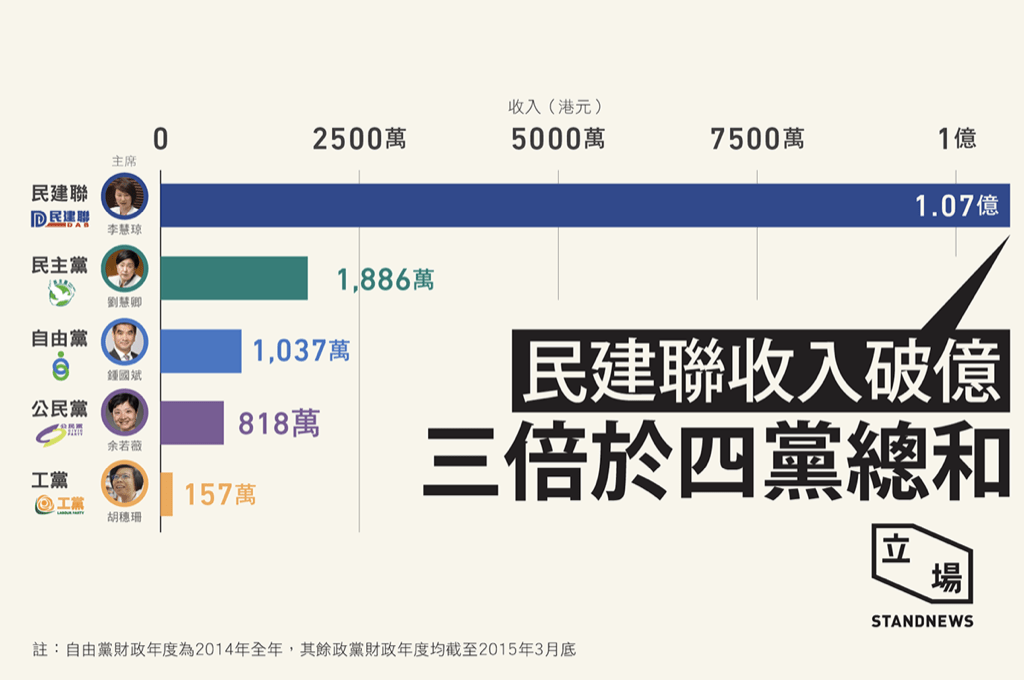
\includegraphics[width=0.7\textwidth]{c33/h-klesson1-053.png}
    \caption{畸型政治格局下政黨面對嚴重資源不均} 
\end{figure}

除捐款外,更直接的干預則是通過利益輸送安排候選人在競爭激烈的選戰中參選,以圖分散非建制陣營的票源。於二零一五年區議會選舉舞弊案中,網台主持鄭永健被控利誘本土派組織參選,打擊傳統民主派的選情。雖然被告被判罪名成立,但審訊過程中有證供指幕後主腦及金主有中方背景,至今仍未查明。

此外,前文提到大眾媒體在九七後的自我審查和政治歸邊也影響到公平競爭(見問題二十八)。例如傳媒可以刻意誇大一些社會議題,然後將之扣為個別政治人物的責任,持續每日跟進報道,即可借新聞採訪的名義行抹黑之實。這些做法有針對非建制陣營的,也有針對建制陣營的。不過考慮到九七以來多數傳媒明顯向建制陣營靠攏,傳媒戰場的不公平競爭同樣明顯,也可視為民主倒退。近年有傳媒持續煽動社會對難民和南亞裔的仇恨,然後經常協助弱勢社群的張超雄議員便被保守輿論攻擊為「難民之父」,正是近年媒體攻擊的例子。

\begin{figure}[htbp]
    \centering
    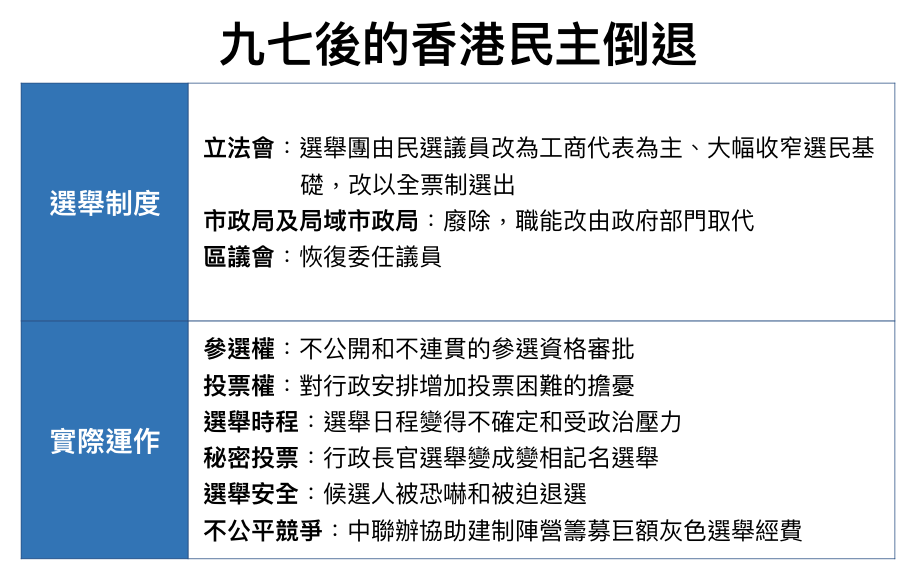
\includegraphics[width=0.7\textwidth]{c33/h-klesson1-055.png}
    \caption{九七後香港民主在制度和實行上都有明顯倒退} 
\end{figure}

最後,現時香港政治問題的核心不僅是九七後的政制是否比九七前更民主,而是當前香港的政制是否落後於社會的實際需要。這點至今已經難以否定。不少香港社會反反覆覆無法解決的問題,無論是住屋、醫療或養老等等,背後都涉及政府缺乏認授無法讓公眾信服,從而展開有力的實質改革。特區成立已有二十二年,社會對政府問責的訴求已經大為提高。無論如何批評九七前的制度不足,也不能合理化今天的政治問題,更不能協助政府解決當前的挑戰。

\rule[-10pt]{15cm}{0.05em}

伸延閱讀:

Fong B (2016) In-between liberal authoritarianism and electoral authoritarianism: Hong Kong’s democratization under Chinese sovereignty, 1997–2016, \textit{Democratization} DOI: 10.1080/13510347.2016.1232249

Poon K (2018) The Impasse Over Constitutional Reform: Negotiating Democracy in Hong Kong, in Fong B and Lui TL (eds) \textit{Hong Kong 20 Years after the Handover: Emerging Social and Institutional Fractures After 1997}, p.3-20.

網上資源:

\href{https://thestandnews.com/politics/政黨財力比恲-民建聯一年收入有幾勁-三倍於民主黨等四黨總收入/}{立場報道(2016):〈民建聯一年收入有幾勁? 三倍於民主黨等四黨總收入〉:立場新聞,2016年2月6日}

\href{https://www.thestandnews.com/politics/周永勤-北京來人說出多名支持者個人資料-威脅-不聽話-棄選就-立即行動/}{立場報道(2016):〈周永勤:北京來人掌握家人支持者個人資料 威脅「不聽話」棄選就「立即行動」〉:立場新聞,2016年9月7日}